\section{问题三模型建立与求解}
\label{sec:question3}

\subsection{问题三分析}

问题三在问题二的日前购电基础上，增加0、6、12、18时发布的未来24小时光伏预报，并允许在规定时点修订尚未执行的常规购电计划。由此产生两个不同的决策频率：常规购电只能按交易时点修订，储能则每10分钟根据实际负荷、光伏与储电量动作。若把两类决策混为每10分钟重新购电，会绕过题目规定的调整费用；若完全照搬日前储能轨迹，又可能在预测误差出现后违反能量平衡。因此，本问采用外层采购、内层执行的双时间尺度结构。

需要先回答三个问题。第一，原计划已经付款，日内增加或减少购电分别意味着什么边际费用；第二，新预报和实测SOC各自能改善哪些决策；第三，规划模型使用的参考储能轨迹，与实际控制器产生的费用是否相同。本问据此保留受交易约束的情景LP作为母模型，在外层加入基于执行规则回放的购电候选筛选，储能仍按原冻结规则执行。最终方案在零时和三个日内修订时点均启用筛选，以开发期闭环账单及筛选时点消融检验其经济性，同时报告紧急补购增加的代价。

\subsection{问题三模型建立}

\subsubsection{结算口径、实际账单与下调支配性}
\label{sec:settlement_mechanism}

记$g_{D,t}$为日期$D$零时承诺的常规购电量，$a_{D,t}$为该时段最后生效的常规购电量，$h_{D,t}$为实际紧急购电量，三者单位均为kWh。设$[x]_+=\max\{x,0\}$。赛题给出计划量计费、1.5倍上调费用、50\%下调违约费及5倍紧急费用，但没有单列取消原计划的退款项。本文采用原计划全额付款且不退款的主解释，并保留退款解释作为敏感性对照。

\begin{table}[htbp]
\centering\small
\caption{问题三两种结算口径及单时段示例（不含紧急购电费）}
\label{tab:mech_settlement_convention}
\begin{tabularx}{\linewidth}{p{0.18\linewidth}Xrr}
\toprule
口径 & 非紧急费用 & 下调示例 & 上调示例\\
\midrule
主口径：不退款 & $pg+1.5p[a-g]_++0.5p[g-a]_+$ & 110元 & 130元\\
退款敏感性口径 & $p\min\{g,a\}+1.5p[a-g]_++0.5p[g-a]_+$ & 90元 & 130元\\
\bottomrule
\end{tabularx}
\par\smallskip\parbox{\linewidth}{\footnotesize 两例均取$g=100$ kWh、$p=1$元/kWh；下调时$a=80$ kWh，上调时$a=120$ kWh。退款解释仅返还取消部分的原计划费用，紧急费用在两种口径下均另加$5ph$。}
\end{table}

主口径的当日真实账单为
\begin{equation}
 C_D=\sum_{t=0}^{143}p_{D,t}\left(g_{D,t}+1.5[a_{D,t}-g_{D,t}]_+
 +0.5[g_{D,t}-a_{D,t}]_++5h_{D,t}\right).
 \label{eq:settlement}
\end{equation}
每次修订均以零时原计划为基准，按最后生效量结算，不把前后两次修订之间的差额重复收费。原计划费用、调整费用及紧急费用分别保存，辅助终端罚项不进入式\eqref{eq:settlement}。

在正电价、原计划不退款、富余电量允许免费弃置三个条件下，下调受到支配。若某可行解$a_t<g_t$，改为$a'_t=g_t$，保持充放电、紧急购电及SOC不变，将多出的$g_t-a_t$弃置，物理约束仍成立，费用却减少$0.5p_t(g_t-a_t)>0$。因而至少存在满足$a_t\ge g_t$的最优解。该结论不适用于退款解释，也不授权内层控制器自行改动已承诺合同。未启用筛选的母模型在两种口径下的334天费用相差320347.51元，故不能把结算语义当作次要实现细节，或因某种解释更便宜而改用该解释。

\subsubsection{由1.5倍增购费用推导条件采购阈值}

沿用问题二的无储能单时段分析，设$X$为修订时未知的实际净需求，$p>0$，并固定原计划$g\ge0$。在主口径下只需考虑$a\ge g$，已承诺的$pg$为常数，因此当前增购决策为
\begin{equation}
 J_3(a)=1.5p(a-g)+5p\,\mathbb E[(X-a)_+],\qquad a\ge g.
 \label{eq:mech_q3_cost}
\end{equation}
其中概率和期望均以该次修订已经获得的信息为条件。设$F_X(x)=\Pr(X\le x)$、$F_X(x^-)=\Pr(X<x)$，则
\begin{equation}
 \partial J_3(a)=p[5F_X(a^-)-3.5,\ 5F_X(a)-3.5].
 \label{eq:q3_adjustment_subgradient}
\end{equation}
内点$a>g$的最优条件为$F_X(a^-)\le0.7\le F_X(a)$，边界$a=g$的最优条件为$F_X(g)\ge0.7$。按下分位数定义，可取
\begin{equation}
 a_3^\star=\max\{g,F_X^{-1}(0.7)\},\qquad
 a_3^\star-g=[F_X^{-1}(0.7)-g]_+.
 \label{eq:mech_q3_quantile}
\end{equation}
离散场景和连续分布均满足上述次梯度刻画；在连续内点，一阶条件也可写为$1.5p-5p\Pr(X>a)=0$。70\%对应给定原计划后的最终有效购电量阈值，既不是增购量本身的分位数，也不是问题三零时计划的最优分位数。储能还引入跨时段库存价值，所以完整调度仍须联合优化，不能逐时套用该解析式。

\subsubsection{合法信息更新与外层滚动采购模型}

用十分钟物理索引表示外层时点，令$\mathcal T_u=\{0,36,72,108\}$。在$\tau\in\mathcal T_u$读取实测储电量$e_\tau^{\rm act}$，只处理$\tau,\ldots,143$的未执行区间；已执行动作及费用保持不变。光伏采用该时点刚发布的预报，负荷零时预测采用一月已选定的最近两个同星期日均值。为利用已经观察到的当天负荷偏差，在$\tau>0$时计算
\begin{align}
 b^L_{D,\tau}&=\frac{1}{12}\sum_{k=\tau-12}^{\tau-1}
       (L_{D,k}-\widehat L^{(0)}_{D,k}),\label{eq:q3_load_bias}\\
 \widehat L^{(\tau)}_{D,t}&=\max\left\{0,\widehat L^{(0)}_{D,t}+
 \operatorname{clip}\!\left(b^L_{D,\tau}e^{-(t-\tau+1)/36},
       -0.3\widehat L^{(0)}_{D,t},0.3\widehat L^{(0)}_{D,t}\right)\right\},\quad t\ge\tau.
 \label{eq:q3_load_update}
\end{align}
$\operatorname{clip}(x,l,u)=\min\{u,\max\{l,x\}\}$。该修正只使用此前两小时实测值，按六小时尺度衰减，并限制在零时预测的$\pm30\%$；这些是预先规定的有限反馈规则，没有用当日未来负荷校准。

在同一发布时间、相同剩余时域内提取此前最多28个完整日的净负荷残差，形成$n_{t,s}$及概率$\pi_s$。保留整日残差片段能表示连续偏高或偏低的误差。母模型在零时求解问题二式\eqref{eq:q2_objective}的经济场景模型；后续时点以已选定的零时计划$g_t$为基准，令$a_t-g_t=u_t^+-u_t^-$，$u_t^+,u_t^-\ge0$，求解
\begin{align}
 \min\quad &\sum_{t=\tau}^{143}\bar p_t(1.5u_t^++0.5u_t^-)
 +\sum_s\pi_s\sum_{t=\tau}^{143}5p_{t,s}h_{t,s}
 +\beta_T|e_{144}-6000|,\label{eq:q3_revision_objective}\\
 \text{s.t.}\quad&a_t+d_t+h_{t,s}-c_t\ge n_{t,s},\quad a_t,h_{t,s}\ge0,
                    \label{eq:q3_revision_balance}\\
 &a_t-g_t=u_t^+-u_t^-,\quad u_t^+,u_t^-\ge0,\quad
 e_\tau=e_\tau^{\rm act},\label{eq:q3_revision_contract}
\end{align}
并满足式\eqref{eq:soc}、\eqref{eq:limits}的储能约束。问题三$p_{t,s}=p_t$为已知分时电价，故$\bar p_t=p_t$；保留场景价格记法便于问题四沿用。原计划费用在当前修订中为常数，可从优化目标略去，但仍计入真实账单。终端系数$\beta_T=\operatorname{median}_{t\ge\tau}\bar p_t$，绝对值通过$e_{144}-6000=z^+-z^-$、$z^+,z^-\ge0$线性化。该项近似剩余库存价值，不强制每天回到6000 kWh。

外层参考充放电和SOC在场景间共享，紧急购电$h_{t,s}$作为场景补救量；主设置预先固定为28场景、无附加风险权重、无参考备用。每次求解当天全部剩余合同，但只把下一合法更新时间之前的部分推进为实际执行量，其后的未执行合同仍可在下个时点按同一规则修订。共享储能限制了策略类，不能把该外层目标直接称为实际控制器的期望费用。

\subsubsection{基于执行规则回放的购电候选筛选}
\label{sec:q3_candidate_screening}

为使采购决策的评估更接近实际执行，在母模型之外建立有限购电候选集合$\mathcal K_\tau$。零时包含五类候选：原情景LP、合法点预测LP，以及净需求预测分别增加$0.25\sigma_t$、$0.5\sigma_t$和$1.0\sigma_t$的三个误差余量LP。其中$\sigma_t^2=\sum_s\pi_s(n_{t,s}-\sum_j\pi_jn_{t,j})^2$，单位为kWh的平方；余量只增加点预测净需求，点预测价格保持不变。日内额外加入“保持当前剩余有效合同”候选，它保留此前修订后尚未执行的合同，并非恢复零时计划。各LP均使用当前同一实测SOC、储能物理约束及零风险、零备用设置，其目标值仅用于产生候选，不能直接跨候选比较。

记候选$k$的剩余常规购电量为$q_t^{(k)}$。对每个候选，从当前共同初态$e_\tau^{\rm act}$出发，在同一组历史情景上按式\eqref{eq:execute_charge}、\eqref{eq:execute_discharge}的固定规则逐段回放，获得$h_{t,s}^{(k)}$与$e_{144,s}^{(k)}$。回放满足$q_t^{(k)}+d_{t,s}^{(k)}+h_{t,s}^{(k)}-c_{t,s}^{(k)}\ge n_{t,s}$，允许富余弃置。所有购电和充放电变量均为电量，附件功率先乘$\Delta t=1/6$ h转换，费用不再重复乘时间步长。剩余时域账单定义为
\begin{align}
 C_{\tau,s}^{\mathrm{replay},(k)}
 &=\sum_{t=\tau}^{143}p_{t,s}\bigl(B_{\tau,t}^{(k)}+5h_{t,s}^{(k)}\bigr),
 \label{eq:q3_replay_bill}\\
 B_{\tau,t}^{(k)}&=
 \begin{cases}
 q_t^{(k)},&\tau=0,\\[1ex]
 g_t+1.5[q_t^{(k)}-g_t]_++0.5[g_t-q_t^{(k)}]_+,&\tau>0.
 \end{cases}\notag
\end{align}
其中$B_{\tau,t}^{(k)}$为以标准电价折算的非紧急计费量。因此，零时按候选计划量全额计费，日内仍计入原计划费，并将最后有效量相对零时计划的调整费完整计入；没有把购电费改成实际使用量的费用。已执行区间对本次选择为常数，不纳入剩余区间评分。

统一评分选择为
\begin{align}
 k_\tau^*&=\arg\min_{k\in\mathcal K_\tau}\sum_s\pi_s
 \left[C_{\tau,s}^{\mathrm{replay},(k)}
 +\beta_\tau\left|e_{144,s}^{(k)}-6000\right|\right],
 \label{eq:q3_candidate_score}\\
 \beta_\tau&=\operatorname{median}_{t\ge\tau}\sum_s\pi_sp_{t,s}.\notag
\end{align}
同一次筛选的情景、权重、初态、执行器、结算规则和终端系数对所有候选相同。末库存偏离项先逐情景计算绝对值再加权，仅用于候选评分，不计入式\eqref{eq:settlement}的实际费用。零时将所选$q^{(k_0^*)}$保存为$g$；日内更新剩余有效合同，并始终以本日$g$为调整基准。评分完全相同时按固定候选顺序选择，优先保留情景LP。

候选回放将当前合同固定至午夜，没有模拟后续尚未发布的预报与合同修订；实际运行仍在下一个合法时点读取新信息并重新决策。因此，这是一种有限候选的执行费用评估，部分改善了规划评估与实际控制的衔接，并非完整多阶段随机最优控制。扩大候选集只能保证同一情景评分下的最小估计费用不增，不能保证未来实际账单下降。最终方案在$\mathcal T_u$的四个时点均启用筛选，适用问题与时点由下文开发性消融确定。

\subsubsection{母模型执行器对照：固定合同内层LP}

母模型与最终增强方案均采用式\eqref{eq:execute_charge}、\eqref{eq:execute_discharge}的规则：富余时在物理上限内充电，缺口时在功率与可用电量允许范围内放电，再紧急补购。该规则仅需当期$a_t,n_t,e_t$，易于执行；但它不直接比较当前与未来电量价值，也不保证跟随外层参考SOC。以下内层LP及跨日续接是基于未启用候选筛选的母模型所作的执行器对照，其结果不作为最终增强方案的同条件消融。

当前时段$t$固定当天剩余常规合同$a_{k|t}$；令当前$\widetilde n_{t|t}=n_t$、$\widetilde p_{t|t}=p_t$，对$k>t$只使用最近合法预报，定义
\begin{equation}
 s_{k|t}=[a_{k|t}-\widetilde n_{k|t}]_+,\qquad
 b_{k|t}=[\widetilde n_{k|t}-a_{k|t}]_+.
 \label{eq:v2_surplus_deficit}
\end{equation}
内层优化为
\begin{align}
 \min\quad&\sum_{k=t}^{143}5\widetilde p_{k|t}(b_{k|t}-d_{k|t})
       +\beta_T|e_{144|t}-6000|,\label{eq:v2_inner_objective}\\
 \text{s.t.}\quad&0\le c_{k|t}\le\min\{U,s_{k|t}\},\quad
 0\le d_{k|t}\le\min\{U,b_{k|t}\},\label{eq:v2_inner_bounds}\\
 &h_{k|t}=b_{k|t}-d_{k|t},\quad
 w_{k|t}=s_{k|t}-c_{k|t},\quad e_{t|t}=e_t^{\rm act},
 \label{eq:v2_inner_balance}
\end{align}
同时满足SOC递推、容量和功率约束。$\beta_T$由当前剩余预测价格的中位数给定。常规合同费用此时不可改变，故从内层目标省略。只执行第一步动作，下一时段获得新实测量后再算；不能在内层增加或取消常规合同。

约束\eqref{eq:v2_inner_bounds}仅允许常规供电富余充电，紧急购电只补负载缺口，不用于主动给电池充电；富余与缺口不能同时为正，故充放电互斥自动成立。与规则执行不同，LP可在预测后续缺口更昂贵时减少当前放电，付出当期补购费以保留电量。作为行为核验，若电池可输出1 kWh、连续两段合同均为0且需求均为1 kWh、电价分别为1与2元/kWh，关闭终端罚项，则规则先放电、后付10元补购；LP先付5元补购、后放电。程序重现了这一机制，但该构造例子不代表全年必然节费。

\subsubsection{母模型执行器对照：跨日预报的续接价值}

6、12、18时公布的是未来24小时预报，分别含次日最初6、12、18小时，即$m=36,72,108$个十分钟段。跨日候选只扩展内层价值估计：次日光伏使用本次已经公布的预报，次日负荷由当日之前已完成的历史日外推；不将当日尚未发生的负荷作为历史样本。零时没有跨日部分，取$m=0$。

当$m>0$时，把固定日末罚项替换为
\begin{equation}
 \widehat V_D(e_{144})=\min_{z,c',d',e'}
 \left\{\sum_{j=0}^{m-1}\widehat p'_jz_j+\beta_T|e'_m-6000|\right\},
 \label{eq:v2_continuation}
\end{equation}
约束为$z_j\ge0$、$z_j+d'_j-c'_j\ge\widehat n'_j$、$e'_0=e_{144}$及相同储能状态方程和物理界。$z_j$为次日临时购电变量，$\beta_T$仍由当天剩余预测价格确定。续接费用使次日需求和补能条件能够影响当前保留库存的价值；这些次日变量不执行、不填入当天购电表、不计入当天真实账单，次日零时再制定正式计划。

该执行器候选仍为确定性续接近似，没有求解次日完整随机交易过程。外层零时模型及候选回放也尚未显式计入以后1.5倍修订的机会：事后允许重新优化，不等于日前已经计算了未来修订的信息价值。严格一致的多阶段策略还需描述合法发布时间上的后续合同修订与信息分支；不能给每条场景独立优化全天储能后直接执行。

\subsection{问题三求解}

\subsubsection{配置确定、滚动实施及费用统计}

先预定经济基准为28场景、风险权重和备用均关闭，再在1月15--31日按实际账单选择预测器与控制候选，不能将风险关闭误写为对风险参数进行一月搜索后的结论。所有同一问题的验证候选从相同实测初态出发，期末库存随候选列出。表\ref{tab:v2_controller_validation}给出未启用候选筛选的母模型在已选预测配置下的控制器验证：问题三规则执行费用919340.82元，剩余日LP为929987.84元，LP加跨日为920497.18元，因而冻结规则执行器。期末库存并不强制相等，这只是有限候选与有限验证期内的选择。预测器与实时执行器沿用这一冻结配置；候选筛选的适用问题及启用时点则依据2--12月开发性回测确定，最终配置确定后固定，本文所报告增强方案结果属于开发期闭环评价。

\begin{table}[htbp]\centering\small
\caption{相同已选预测配置下的执行器一月验证}
\label{tab:v2_controller_validation}
\begin{tabularx}{\linewidth}{LLRRR}\toprule
问题 & 执行器 & 实际费用/元 & 紧急量/kWh & 末库存/kWh\\\midrule
问题2 & 规则执行 & 917318.59 & 19.93 & 7155.31\\
问题2 & 储能LP & 928995.30 & 474.33 & 6000.00\\
问题3 & 规则执行 & 919340.82 & 49.23 & 7143.30\\
问题3 & 储能LP & 929987.84 & 195.13 & 6000.00\\
问题3 & 储能LP+跨日 & 920497.18 & 195.13 & 7143.30\\
问题4-2 & 规则执行 & 1042234.20 & 19.93 & 7298.41\\
问题4-2 & 储能LP & 1052652.76 & 19.93 & 6000.00\\
问题4-3 & 规则执行 & 1043044.13 & 44.10 & 7308.72\\
问题4-3 & 储能LP & 1057597.78 & 220.05 & 6000.00\\
问题4-3 & 储能LP+跨日 & 1047012.91 & 220.05 & 7291.46\\
\bottomrule\end{tabularx}
\par\smallskip\parbox{\linewidth}{\footnotesize 同一问题内使用相同1月15日期初库存，之后独立因果运行。费用不含终端罚项；末库存并不强制相等。}
\end{table}

实际求解使用稀疏LP和HiGHS。每日流程为：零时读取合法预报与承接SOC，生成购电候选并按式\eqref{eq:q3_candidate_score}筛选原计划；每10分钟读取当前实值并按固定规则执行储能；到6、12、18时用实测SOC和新信息生成并筛选未执行采购段，其中保留当前合同候选；日末按式\eqref{eq:settlement}分项结算，并令$e_{D+1,0}=e_{D,144}$。原版已执行的一月轨迹作为固定前缀，同一问题的母模型、最终方案及对照从相同2月初态开始，之后独立、连续推进状态，不能用后来选定的配置回写一月，也不每日重置库存。

问题三最终方案2月初态为8814.60 kWh，12月末为6240.32 kWh。334天计划费13503057.82元、调整费248699.70元、紧急费119713.93元，总费用13871471.44元。紧急购电21029.90 kWh，涉及119天、424个十分钟段；经紧急补购后逐段满足负载，紧急量不代表失供电量。实际日账单CVaR95为65552.76元，最高日费用为67941.61元。与保留母模型的问题二横向比较，总费用低1.0086\%、紧急量低75.26\%，但两问的零时光伏来源、初态和采购配置不同，不能把全部差异归为滚动反馈的独立作用。

\subsubsection{筛选时点消融与最终策略选择}
\label{sec:q3_screening_ablation}

为考察候选筛选在不同决策阶段的作用，在保持预测方法、历史情景构造、实时执行器、结算规则及合法采购修订时点不变的条件下，设置不启用筛选、仅零时筛选、仅日内筛选及零时与日内均筛选四种配置。关闭筛选的时点仍调用母模型情景LP，使用该方案自身的实测SOC与零时计划重新优化；“仅零时筛选”仍保留6、12、18时的合法预测更新和采购修订，并不等于仅制定一次日前计划。各组从同一问题的共同初态连续运行，以计划费用、调整费用和紧急费用之和评价，不将评分终端项计入实际账单。

\begin{table}[htbp]\centering\small
\caption{候选筛选启用时点对实际总费用的影响}
\label{tab:outer_timing_ablation}
\begin{tabularx}{\linewidth}{LRR}\toprule
候选筛选配置 & 问题3总费用/元 & 问题4滚动版总费用/元\\\midrule
不启用筛选：母模型基线 & 13,975,810.86 & 14,769,232.53\\
仅零时启用 & 13,911,957.70 & 14,712,596.45\\
仅日内启用 & 13,947,087.88 & 14,734,593.23\\
\textbf{零时＋日内均启用：最终方案} & \textbf{13,871,471.44} & \textbf{14,670,237.87}\\
\bottomrule\end{tabularx}
\par\smallskip\parbox{\linewidth}{\footnotesize 各组均保留0、6、12、18时的合法预报更新与采购修订，仅改变是否启用候选筛选；关闭筛选时仍调用原情景优化模型。各方案从同一问题的共同初态出发，之后独立、连续推进状态，不每日重置。评价范围为2025年2月1日至12月31日，共334天。}
\end{table}


在2025年2月1日至12月31日的334天开发性闭环回测中，全时点筛选在表\ref{tab:outer_timing_ablation}的四种配置中费用最低。第三问相较未启用筛选的母模型13975810.86元节省104339.41元，降幅0.747\%；相较仅零时和仅日内筛选，分别进一步节省40486.25元和75616.44元。第四问滚动版全时点费用14670237.87元，相较其母模型节省98994.66元，降幅0.670\%；相较仅零时和仅日内筛选，分别进一步节省42358.58元和64355.36元。差值由未舍入账单计算。这些结果支持在本次比较的四种配置中保留全时点筛选，不证明其在任意数据或候选集合下均最优。

\begin{table}[htbp]\centering\small
\caption{滚动采购候选筛选的费用与紧急补购权衡}
\label{tab:outer_screening_tradeoff}
\begin{tabularx}{\linewidth}{LLRRRR}\toprule
问题 & 配置 & 计划费/万元 & 调整费/万元 & 紧急费/万元 & 紧急量/kWh\\\midrule
问题3 & 母模型 & 1367.46 & 23.07 & 7.06 & 12647.76\\
问题3 & 最终方案 & 1350.31 & 24.87 & 11.97 & 21029.90\\
问题4滚动版 & 母模型 & 1446.02 & 24.19 & 6.71 & 11950.68\\
问题4滚动版 & 最终方案 & 1426.52 & 28.31 & 12.19 & 21293.41\\
\bottomrule\end{tabularx}
\par\smallskip\parbox{\linewidth}{\footnotesize 计划费按零时计划量全额结算，调整费始终以零时原计划为基准；紧急购电单独计费。终端偏离项不计入实际账单。两问题均以计划费用下降补偿新增调整费与紧急费。}
\end{table}


同一问题四组方案的评价期末库存一致，第三问均为6240.32 kWh、第四问滚动版均为6274.99 kWh，因此费用排序不能由期末额外消耗库存解释。但表\ref{tab:outer_screening_tradeoff}也显示，经济性改善伴随更多紧急补购：第三问紧急量由12647.76增至21029.90 kWh，第四问滚动版由11950.68增至21293.41 kWh。第三问计划费减少171508.13元，超过新增调整费18034.75元与紧急费49133.97元；第四问滚动版计划费减少195001.12元，超过新增调整费41200.07元与紧急费54806.39元。收益来自账单三项的净变化，并非所有运行指标同时改善。

同一候选模块用于问题二和第四问日前版时，费用反而分别增加22571.98元（0.161\%）和63356.15元（0.428\%），因此这两组仍采用母模型。最终分问配置为“日前两组不筛选、滚动两组零时与日内均筛选”。逐决策检查验证了当时可用信息边界、同口径评分和连续执行，但这种因果可执行性不等于模型选型没有参考回测结果；上述结论属于开发期选型证据，不是未接触数据上的独立测试，也不提供未来费用或跨年份最优性保证。

\subsubsection{状态、新光伏及负荷反馈的逐层贡献}

为分开信息来源，以下保留基于未启用候选筛选的母模型所作的独立消融。在相同初态、场景设定和规则控制器下，依次比较仅零时外层计划、只更新SOC并按零时预测重优化、再加入新光伏预报、最后加入已观测负荷偏差修正。四组均关闭候选筛选与跨日续接，避免“SOC-only”组从次日光伏预报间接获得新信息；每组之后按自身状态与合同因果演化。此实验考察信息来源，表\ref{tab:outer_timing_ablation}考察筛选模块的启用位置，两者配置与问题不同，不能相互替代。

\begin{table}[htbp]\centering\small
\caption{问题3母模型的状态、光伏和负荷反馈分解}
\label{tab:v2_feedback}
\begin{tabularx}{\linewidth}{LRRRR}\toprule
策略 & 总费/万元 & 紧急量/kWh & 日费CVaR95/元 & 末库存/kWh\\\midrule
仅零时外层计划 & 1416.90 & 80181.62 & 71801.23 & 6240.32\\
仅更新SOC并重优化 & 1399.17 & 39298.96 & 66748.14 & 6240.32\\
再加入新光伏预报 & 1407.57 & 40071.16 & 66732.97 & 6240.32\\
再加入负荷偏差反馈 & 1397.58 & 12647.76 & 65518.79 & 6240.32\\
\bottomrule\end{tabularx}
\par\smallskip\parbox{\linewidth}{\footnotesize 本表基于未启用候选筛选的母模型，各组保留原实验配置及数值，覆盖相同334天并连续推进状态；不作为最终筛选算法的同条件消融。}
\end{table}


仅零时外层计划费用14169011.89元，更新SOC后降至13991697.93元，减少177313.97元；再加入新光伏后增至14075665.67元，增加83967.74元；继续加入负荷偏差反馈后降至母模型基线13975810.86元，减少99854.81元。图\ref{fig:q3-feedback-waterfall}将这三项增量与起止账单分开显示。新信息的经济价值取决于采购、储能状态与误差的共同作用，不能预先认定每份新预报都节费。附件没有提供其他发布时间的预报，不用实际未来光伏代替不存在的高频预报来构造所谓实测收益。

\begin{figure}[htbp]\centering
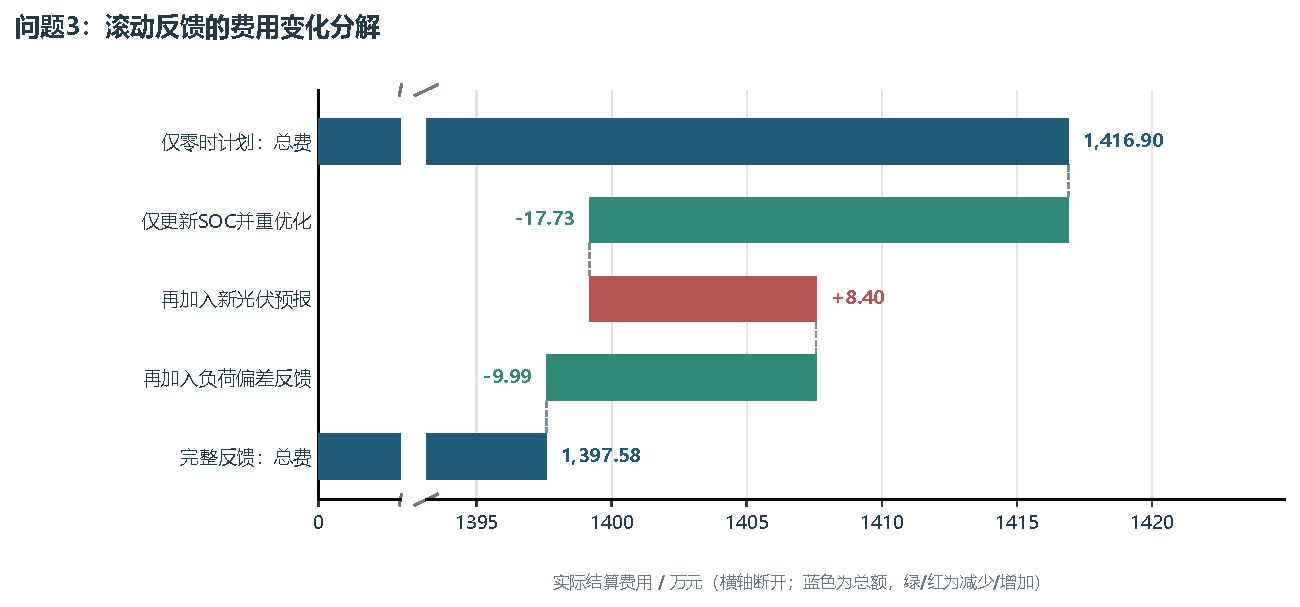
\includegraphics[width=0.94\linewidth]{figures/results/q3_feedback_waterfall.pdf}
\caption{未启用候选筛选的母模型逐层反馈费用分解。横轴单位为万元，断轴用于放大账单附近的差异，起止条从零累计至334天总账单，中间条为相邻策略的费用差；增量包含各自闭环状态与后续采购的共同响应，不是单次预报的独立因果效应。}
\label{fig:q3-feedback-waterfall}
\end{figure}

\subsubsection{同计划回放：规划与控制的偏差}

本节分别考察原版12场景配置与未启用筛选的28场景母模型的规划与执行差异，诊断结果限于各自原有配置。原版采用12代表场景、自适应风险基数0.1和备用系数1，未启用候选筛选。重解全年3650个外层决策点，重建购电量在实际执行区间与保存结果完全相同。固定计划、初态与历史场景逐步回放，定义
\begin{equation}
 \Delta_{\rm exec}=\sum_s\pi_s\left(C_s^{\rm replay}-C_s^{\rm plan}\right).
 \label{eq:v2_execution_gap}
\end{equation}
两种费用都只含常规采购、调整及紧急采购，排除CVaR、终端罚项和数值破同解项。表\ref{tab:v2_execution_gap}汇总2--12月各决策点：原版问题二、三、四静态、四滚动的平均偏差依次为$-986.50$、$-569.90$、$-1068.47$、$-582.32$元。

\begin{table}[htbp]\centering\small
\caption{原版同计划、同初态、同场景的规划与执行偏差}
\label{tab:v2_execution_gap}
\begin{tabularx}{\linewidth}{LRRRR}\toprule
问题 & 决策点数 & 平均$\Delta_{\rm exec}$/元 & 负偏差比例 & SOC均方根偏差/kWh\\\midrule
问题2 & 334 & -986.50 & 97.90\% & 1319.72\\
问题3 & 1336 & -569.90 & 94.24\% & 994.32\\
问题4-2 & 334 & -1068.47 & 99.40\% & 1350.69\\
问题4-3 & 1336 & -582.32 & 93.94\% & 1048.30\\
\bottomrule\end{tabularx}
\par\smallskip\parbox{\linewidth}{\footnotesize 每一决策点先按场景概率计算费用差与SOC均方根偏差，再对决策点取均值；滚动剩余时域相互重叠，不将这些差求和解释为年度费用。全部费用仅计实际结算项目。}
\end{table}

负偏差不说明原规划已经正确描述控制，而是参考储能跨场景共享，实际规则可以利用当前观测改变动作，回放费用因此可能更低；正偏差也会出现。诊断窗口为剩余日，滚动窗口相互重叠，不能把差值相加成年度节费，也不能称其为相对全局最优的差距。图\ref{fig:q3-execution-band}取原版问题三正费用偏差最大的2025年2月9日零时决策，展示同一合同下12条历史场景的规则回放。此图来自保留个体轨迹的原版数据，与下文28场景母模型的16点双控制器诊断分开解释。

\begin{figure}[htbp]\centering
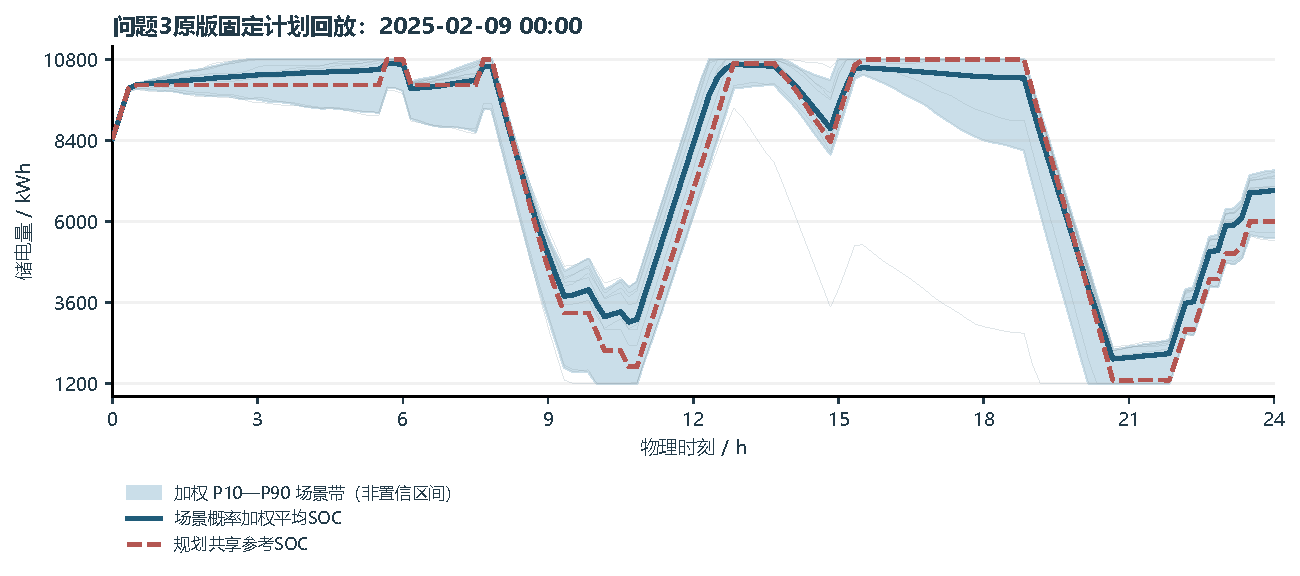
\includegraphics[width=0.95\linewidth]{figures/results/q3_execution_band.pdf}
\caption{原版问题三2025年2月9日零时同一合同下的12场景规则回放。虚线为共享参考SOC，实线为场景概率加权均值，细灰线为个体场景；阴影为各时刻按原概率计算的P10--P90加权经验分位带，不是置信区间或全年覆盖保证。图中不含内层LP轨迹。}
\label{fig:q3-execution-band}
\end{figure}

进一步在未启用筛选的28场景母模型上，对问题三4个指定日、4个外层时点，共16个决策点固定同一合同、实际初态与历史场景，对规则和内层LP各回放448条轨迹。每一步只揭示该步场景净需求和价格，未来仍使用该决策点已合法获得的点预测；后续合同和预报不再更新。这一计算分离了同一计划下换控制器的影响，以及全年闭环运行导致后续计划也改变的影响。

\begin{table}[htbp]\centering\small
\caption{未筛选母模型计划下两种执行器的回放诊断}
\label{tab:v2_inner_gap}
\begin{tabularx}{\linewidth}{LRR}\toprule
指标 & 规则执行 & 内层LP\\\midrule
有符号期望费用偏差/元 & -655.33 & -513.41\\
场景费用绝对偏差的期望/元 & 697.25 & 605.16\\
SOC均方根偏差/kWh & 1056.40 & 869.79\\
\bottomrule\end{tabularx}
\par\smallskip\parbox{\linewidth}{\footnotesize 四个指定日、四个时点共16个决策点，每点28场景。先计算场景概率加权指标，再对决策点等权平均；两种执行器固定相同购电合同和初态，仅逐步揭示当前场景值。}
\end{table}


平均SOC均方根偏差由规则执行1056.40 kWh降至内层LP的869.79 kWh，场景费用绝对偏差的期望由697.25元降至605.16元，但LP每个决策点的平均回放账单反而增加141.92元。16点中，10点的绝对期望费用偏差减小，仅1点的实际回放费用更低。更接近参考轨迹是一项可观察改善，却不能替代经济目标。最终增强方案由原执行器直接回放采购候选以缓解这一评估差异，但受剩余日固定合同近似所限，仍未达到严格多阶段一致。

\subsubsection{母模型内层LP与跨日续接的全年检验}

本节各组均未启用候选筛选，保持原有执行器对照配置。

\begin{table}[htbp]\centering\small
\caption{问题3母模型的执行控制与跨日续接对照}
\label{tab:v2_controllers}
\begin{tabularx}{\linewidth}{LRRRR}\toprule
策略 & 总费/万元 & 紧急量/kWh & 日费CVaR95/元 & 末库存/kWh\\\midrule
规则执行（母模型） & 1397.58 & 12647.76 & 65518.79 & 6240.32\\
剩余日储能LP & 1421.32 & 23825.27 & 66397.37 & 5934.55\\
储能LP+跨日价值 & 1405.26 & 22407.53 & 66033.05 & 6240.32\\
\bottomrule\end{tabularx}
\par\smallskip\parbox{\linewidth}{\footnotesize 本表基于未启用候选筛选的母模型，各组保留原实验配置及数值，覆盖相同334天并连续推进状态；不作为最终筛选算法的同条件消融。}
\end{table}


在334天完整闭环中，仅将母模型规则执行器换成剩余日LP，费用为14213193.28元，比规则母模型增加237382.42元，紧急量也增至23825.27 kWh。该候选将外层共享参考储能与内层有限点预测组合使用，并不必然优化真实未来费用，因此不予采用。

在相同LP下启用合法跨日信息后，费用降至14052638.61元，比截断于午夜的LP少160554.67元，紧急量少1417.74 kWh，年末库存还增加305.77 kWh。跨日改善并非依靠更多放空电池取得，但它仍比规则母模型多付76827.75元。控制器和续接候选均保持一月后的设置冻结，不依据评价期费用重新选择执行器；外层候选筛选的开发期选型另见第\ref{sec:q3_screening_ablation}节。

\subsubsection{退款口径的独立敏感性}

固定未启用候选筛选的母模型的预测、场景、控制器和初态，仅切换表\ref{tab:mech_settlement_convention}中的退款解释并重新优化，按各自规则结算。该比较检验制度语义，既不改变附件主口径，也不计作算法节费；表中不退款基线仍为13975810.86元，不与最终筛选方案混列。

\begin{table}[htbp]\centering\small
\caption{问题3母模型的结算解释敏感性}
\label{tab:v2_settlement}
\begin{tabularx}{\linewidth}{LRRRR}\toprule
策略 & 总费/万元 & 紧急量/kWh & 日费CVaR95/元 & 末库存/kWh\\\midrule
主口径：不退款 & 1397.58 & 12647.76 & 65518.79 & 6240.32\\
取消部分退款 & 1365.55 & 12871.85 & 64278.33 & 6240.32\\
\bottomrule\end{tabularx}
\par\smallskip\parbox{\linewidth}{\footnotesize 本表基于未启用候选筛选的母模型，各组保留原实验配置及数值，覆盖相同334天并连续推进状态；不作为最终筛选算法的同条件消融。}
\end{table}


退款解释费用13655463.35元，比不退款主口径少320347.51元，累计下调1096916.99 kWh，净调整费用为$-113349.02$元。两组年末库存相同，差异来自费用规则和对应采购响应，其量级大于若干模型增强的收益。退款后取消采购的边际费用改变，下调可以为正；不能再使用不退款条件下的支配结论。

\subsubsection{指定日期结果与实际运行轨迹}

图\ref{fig:v2-control}取最终方案评价期紧急量最大日7月4日，将最终上调量、实际SOC及紧急量分开呈现；库存子图同时给出未启用筛选的母模型实际SOC，便于观察不同采购决策形成的连续状态轨迹。两条曲线均来自各自实际执行数组。图\ref{fig:v2-adjustments}另列最终方案四个指定日的$a_t-g_t$，避免两条大部分重合的购电总量曲线遮盖修订。

\begin{figure}[htbp]\centering
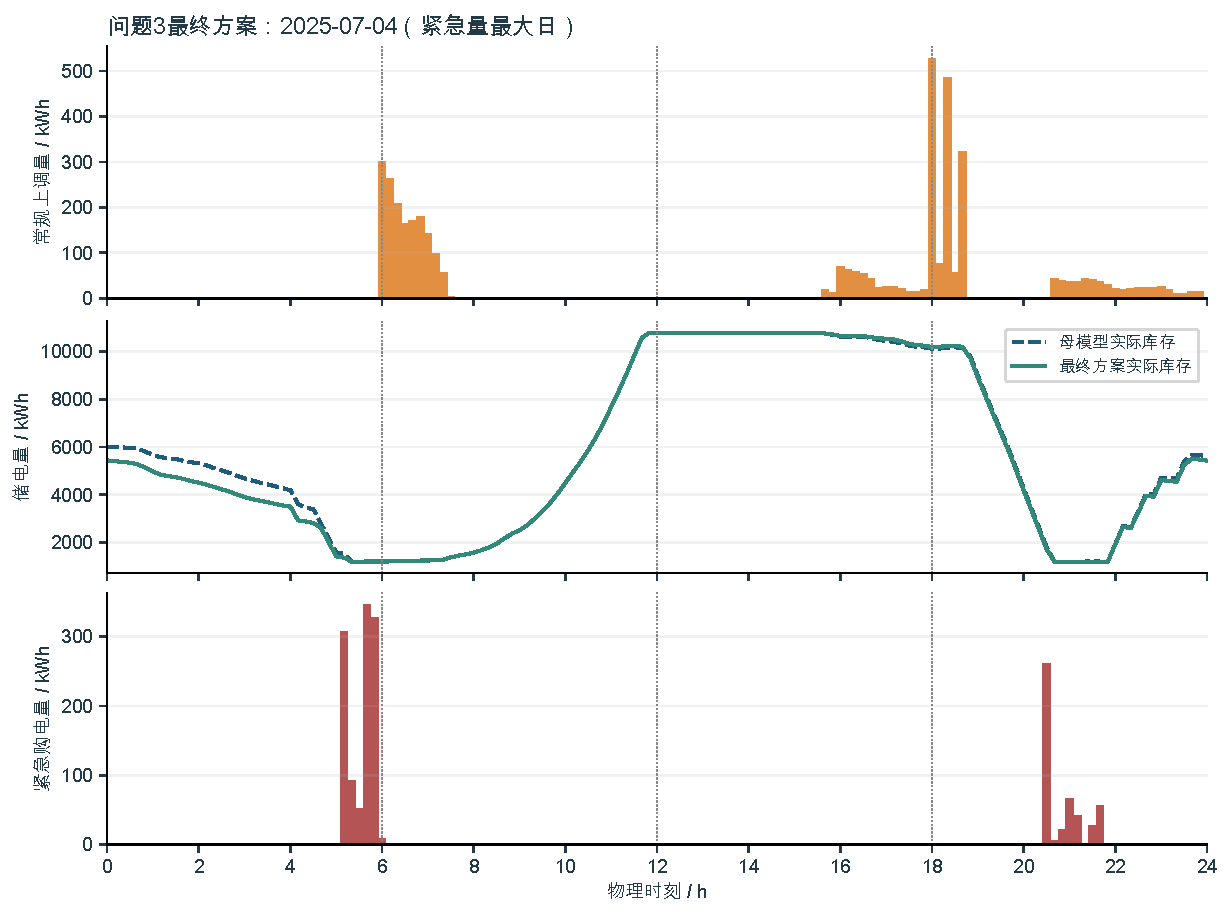
\includegraphics[width=0.95\linewidth]{figures/results/v2_control_difference.pdf}
\caption{问题三最终方案紧急量最大日的购电调整、实际SOC与紧急购电。库存子图比较最终方案与未筛选母模型各自的实际SOC；虚线标示6、12、18时的日内修订时点，实际状态连续传递。}
\label{fig:v2-control}
\end{figure}
\begin{figure}[htbp]\centering
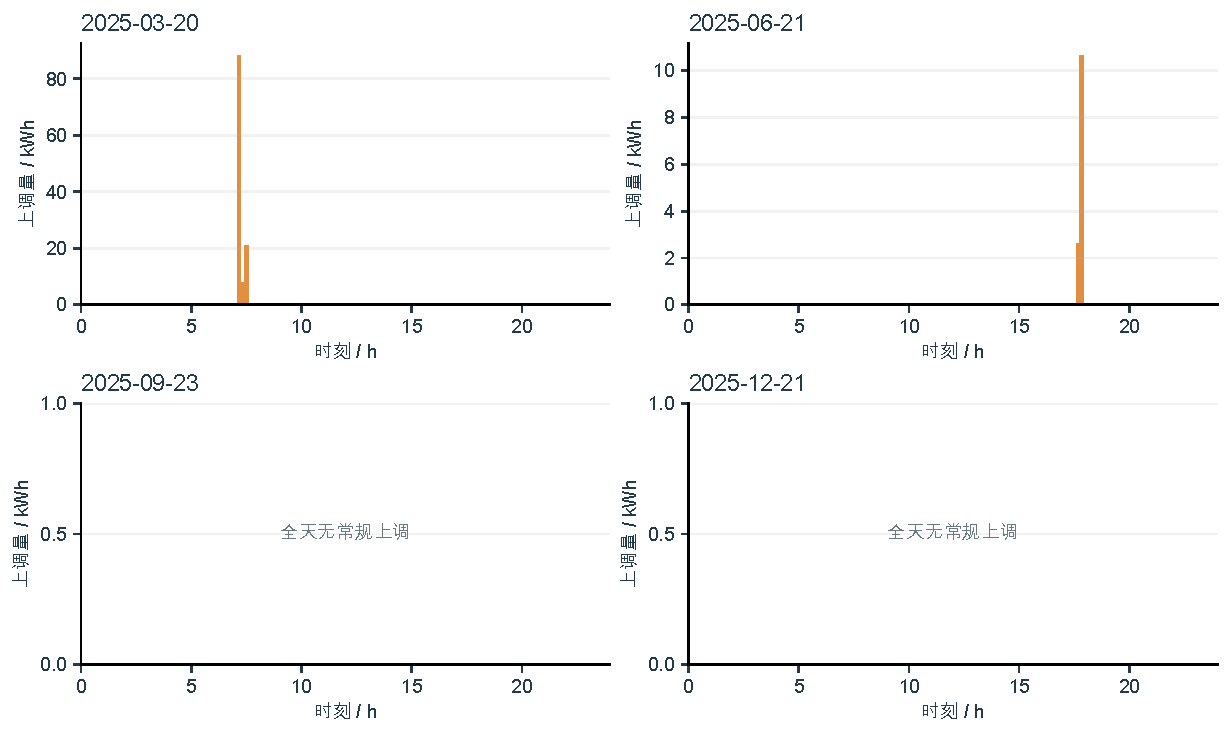
\includegraphics[width=0.95\linewidth]{figures/results/v2_adjustments.pdf}
\caption{最终方案四个指定日期最后生效常规购电量与零时计划之差$a_t-g_t$。数据来自全时点筛选的实际执行数组，不含紧急购电量；无调整时差值为零。}
\label{fig:v2-adjustments}
\end{figure}

\begin{table}[htbp]\centering\small
\caption{问题3指定日期购电结果（沿用题目表1布局，电量单位：kWh）}
\label{tab:q3-purchase}
\par\smallskip\textbf{2025-03-20}\par\smallskip
\begin{tabularx}{\linewidth}{lRlRlR}
\toprule
时间段 & 购电量 & 时间段 & 购电量 & 时间段 & 购电量\\
\midrule
10:00--10:10 & 0.00 & 12:00--12:10 & 624.29 & 14:00--14:10 & 0.00\\
16:00--16:10 & 671.04 & 18:00--18:10 & 704.20 & 20:00--20:10 & 0.00\\
\midrule
全天购电量 & 71789.01 & \multicolumn{2}{c}{全天购电费（元）} & \multicolumn{2}{r}{45563.84}\\
\bottomrule
\end{tabularx}
\par\smallskip\textbf{2025-06-21}\par\smallskip
\begin{tabularx}{\linewidth}{lRlRlR}
\toprule
时间段 & 购电量 & 时间段 & 购电量 & 时间段 & 购电量\\
\midrule
10:00--10:10 & 0.00 & 12:00--12:10 & 0.00 & 14:00--14:10 & 0.00\\
16:00--16:10 & 260.52 & 18:00--18:10 & 0.00 & 20:00--20:10 & 0.00\\
\midrule
全天购电量 & 37273.13 & \multicolumn{2}{c}{全天购电费（元）} & \multicolumn{2}{r}{21986.55}\\
\bottomrule
\end{tabularx}
\par\smallskip\textbf{2025-09-23}\par\smallskip
\begin{tabularx}{\linewidth}{lRlRlR}
\toprule
时间段 & 购电量 & 时间段 & 购电量 & 时间段 & 购电量\\
\midrule
10:00--10:10 & 0.00 & 12:00--12:10 & 444.81 & 14:00--14:10 & 0.00\\
16:00--16:10 & 611.01 & 18:00--18:10 & 801.37 & 20:00--20:10 & 0.00\\
\midrule
全天购电量 & 73472.67 & \multicolumn{2}{c}{全天购电费（元）} & \multicolumn{2}{r}{46201.57}\\
\bottomrule
\end{tabularx}
\par\smallskip\textbf{2025-12-21}\par\smallskip
\begin{tabularx}{\linewidth}{lRlRlR}
\toprule
时间段 & 购电量 & 时间段 & 购电量 & 时间段 & 购电量\\
\midrule
10:00--10:10 & 0.00 & 12:00--12:10 & 1054.19 & 14:00--14:10 & 0.00\\
16:00--16:10 & 877.48 & 18:00--18:10 & 744.23 & 20:00--20:10 & 0.00\\
\midrule
全天购电量 & 101747.42 & \multicolumn{2}{c}{全天购电费（元）} & \multicolumn{2}{r}{65702.81}\\
\bottomrule
\end{tabularx}
\par\smallskip\parbox{\linewidth}{\footnotesize 注：问题2与4-2列示计划购电量；问题3与4-3列示最终生效的调整后常规购电量。全天购电量不含紧急购电，全天购电费含计划、调整与紧急费用。}
\end{table}

\begin{table}[htbp]\centering\small
\caption{问题3指定日期储能结果（沿用题目表2布局，单位：kWh）}
\label{tab:q3-battery}
\par\smallskip\textbf{2025-03-20}\par\smallskip
\begin{tabularx}{\linewidth}{lRRlRR}
\toprule
时间段 & 充电量 & 放电量 & 时间段 & 充电量 & 放电量\\
\midrule
00:00--04:00 & 4146.19 & 181.53 & 04:00--08:00 & 883.67 & 6201.85\\
08:00--12:00 & 5765.88 & 2465.92 & 12:00--16:00 & 5215.25 & 254.72\\
16:00--20:00 & 1.31 & 5594.70 & 20:00--24:00 & 5703.85 & 2960.43\\
\midrule
0:00储电量 & \multicolumn{2}{r}{6505.69} & 24:00储电量 & \multicolumn{2}{r}{6428.95}\\
\bottomrule
\end{tabularx}
\par\smallskip\textbf{2025-06-21}\par\smallskip
\begin{tabularx}{\linewidth}{lRRlRR}
\toprule
时间段 & 充电量 & 放电量 & 时间段 & 充电量 & 放电量\\
\midrule
00:00--04:00 & 915.21 & 972.82 & 04:00--08:00 & 511.20 & 4390.39\\
08:00--12:00 & 8439.30 & 0.00 & 12:00--16:00 & 0.00 & 0.00\\
16:00--20:00 & 241.25 & 5157.72 & 20:00--24:00 & 6354.48 & 2485.90\\
\midrule
0:00储电量 & \multicolumn{2}{r}{7879.99} & 24:00储电量 & \multicolumn{2}{r}{8243.25}\\
\bottomrule
\end{tabularx}
\par\smallskip\textbf{2025-09-23}\par\smallskip
\begin{tabularx}{\linewidth}{lRRlRR}
\toprule
时间段 & 充电量 & 放电量 & 时间段 & 充电量 & 放电量\\
\midrule
00:00--04:00 & 4692.99 & 53.14 & 04:00--08:00 & 892.10 & 5612.58\\
08:00--12:00 & 6293.08 & 1896.62 & 12:00--16:00 & 3282.98 & 403.62\\
16:00--20:00 & 15.07 & 5619.05 & 20:00--24:00 & 5609.40 & 3045.21\\
\midrule
0:00储电量 & \multicolumn{2}{r}{6006.02} & 24:00储电量 & \multicolumn{2}{r}{6235.06}\\
\bottomrule
\end{tabularx}
\par\smallskip\textbf{2025-12-21}\par\smallskip
\begin{tabularx}{\linewidth}{lRRlRR}
\toprule
时间段 & 充电量 & 放电量 & 时间段 & 充电量 & 放电量\\
\midrule
00:00--04:00 & 4496.41 & 40.16 & 04:00--08:00 & 762.28 & 1406.28\\
08:00--12:00 & 6441.76 & 6526.43 & 12:00--16:00 & 5333.82 & 2222.97\\
16:00--20:00 & 0.00 & 5526.27 & 20:00--24:00 & 5771.81 & 2842.53\\
\midrule
0:00储电量 & \multicolumn{2}{r}{6797.85} & 24:00储电量 & \multicolumn{2}{r}{6695.97}\\
\bottomrule
\end{tabularx}
\end{table}

\begin{table}[htbp]\centering\small
\caption{问题3指定日期紧急购电（题目表3布局，单位：kWh）}
\label{tab:q3-emergency}
\setlength{\tabcolsep}{3pt}
\begin{tabularx}{\linewidth}{lRlRlRlR}\toprule
\multicolumn{2}{c}{2025-03-20} & \multicolumn{2}{c}{2025-06-21} & \multicolumn{2}{c}{2025-09-23} & \multicolumn{2}{c}{2025-12-21}\\
时间段 & 购电量 & 时间段 & 购电量 & 时间段 & 购电量 & 时间段 & 购电量\\\midrule
09:10--10:00 & 311.46 & 无 & 0.00 & 20:20--20:30 & 6.38 & 无 & 0.00\\
 &   &  &   & 20:50--21:10 & 67.74 &  &  \\
 &   &  &   & 21:20--21:50 & 34.20 &  &  \\
\midrule
合计 & 311.46 & 合计 & 0.00 & 合计 & 108.31 & 合计 & 0.00\\
\bottomrule\end{tabularx}\end{table}
\begin{table}[htbp]\centering\small
\caption{问题3指定日期计划、调整与费用分解}
\begin{tabularx}{\linewidth}{lRRRRR}\toprule
日期 & 计划量/kWh & 生效量/kWh & 计划费/元 & 调整费/元 & 紧急费/元\\\midrule
2025-03-20 & 71671.98 & 71789.01 & 43906.14 & 136.18 & 1521.51\\
2025-06-21 & 37259.86 & 37273.13 & 21962.65 & 23.90 & 0.00\\
2025-09-23 & 73472.67 & 73472.67 & 45684.65 & 0.00 & 516.92\\
2025-12-21 & 101747.42 & 101747.42 & 65702.81 & 0.00 & 0.00\\
\bottomrule\end{tabularx}\end{table}

以上指定日期表、运行轨迹及全年工作簿均由最终全时点筛选的同一执行数组生成。指定时段和紧急区间按统一物理索引生成，四小时充放电量按其中24个十分钟段合计。一个四小时区间内充、放电量同时为正，可以表示不同十分钟时段分别充电和放电。计划页保存原计划费用，调整页保存最后生效的常规量及完整实际费用；不把辅助目标值填成实际账单。
\FloatBarrier
